% arara: pdflatex
% arara: biber
% arara: pdflatex
% arara: pdflatex

\documentclass{beamer}
\usetheme{Luebeck}
\usecolortheme{crane}
\usepackage[backend=biber,style=authoryear-comp,useprefix=false]{biblatex}

\usepackage{stmaryrd}
\usepackage[]{amsmath}
\usepackage{amsfonts}
\usepackage{amssymb}
\usepackage{mathtools}
\usepackage{forest}
\usepackage{tabularx}
\usepackage{linguex}
\usepackage{centernot}
\usepackage{todonotes}
\useforestlibrary{linguistics}

\forestset{tree defaults/.style={for tree={parent anchor=south, child anchor=north},every tree node/.style={align=center,anchor=north},level/.style={sibling distance=50mm/#1},baseline}}

\forestset{en/.style={parent anchor=center, child anchor=center}}
\forestset{em/.style={parent anchor=north west, child anchor=north west}}
\forestset{el/.style={parent anchor=north, child anchor=north}}

\usetikzlibrary{positioning}
\usetikzlibrary{calc}
\usetikzlibrary{arrows}
\usetikzlibrary{decorations.markings}
%\DeclareNameFormat{labelname:poss}{% Based on labelname from biblatex.def
%  \ifcase\value{uniquename}%
%  \usebibmacro{name:last}{#1}{#3}{#5}{#7}%
%  \or
%  \ifuseprefix
%  {\usebibmacro{name:first-last}{#1}{#4}{#5}{#8}}
%  {\usebibmacro{name:first-last}{#1}{#4}{#6}{#8}}%
%  \or
%  \usebibmacro{name:first-last}{#1}{#3}{#5}{#7}%
%  \fi
%  \usebibmacro{name:andothers}%
%  \ifnumequal{\value{listcount}}{\value{liststop}}{'s}{}
%}
%
%\DeclareFieldFormat{shorthand:poss}{%
%  \ifnameundef{labelname}{#1's}{#1}
%}
%
%\DeclareFieldFormat{citetitle:poss}{\mkbibemph{#1}'s}
%
%\DeclareFieldFormat{label:poss}{#1's}
%
%\newrobustcmd*{\posscitealias}{%
%  \AtNextCite{%
%    \DeclareNameAlias{labelname}{labelname:poss}%
%    \DeclareFieldAlias{shorthand}{shorthand:poss}%
%    \DeclareFieldAlias{citetitle}{citetitle:poss}%
%    \DeclareFieldAlias{label}{label:poss}
%  }
%}
%
%\newrobustcmd*{\posscite}{%
%  \posscitealias%
%  \textcite
%}
%
%\newrobustcmd*{\Posscite}{\bibsentence\posscite}
%
%\newrobustcmd*{\posscites}{%
%  \posscitealias%
%  \textcites
%}

\newcommand\quelle[1]{{%
  \unskip\nobreak\hfil\penalty50
  \hskip2em\hbox{}\nobreak\hfil#1%
  \parfillskip=0pt \finalhyphendemerits=0 \par
}
}

\newcommand{\figex}{\refstepcounter{ExNo}\theExNo\hspace{\Exlabelsep}}

\newcounter{DerivStep}

\newcommand{\hxp}{$\left\{ \text{X, YP} \right\}$}
\newcommand{\hh}{$\left\{ \text{X, Y} \right\}$}
\newcommand{\xpyp}{$\left\{ \text{XP, YP} \right\}$}
\bibliography{Thesis}
%\AtBeginSection[]
%{
%  \begin{frame}
%    \frametitle{Table of Contents}
%    \tableofcontents[currentsection]
%  \end{frame}
%}
\title{Explaining the Resultative Parameter}
\subtitle{Thesis Proposal}
\author{Dan Milway}
\begin{document}
\section{}
\frame[plain]{\titlepage}
\section{What is the Resultative Parameter?}
\begin{frame}
  \vfill
  \centering
  \begin{beamercolorbox}[sep=8pt,center]{title}
    \usebeamerfont{title}
    What is the Resultative Parameter?
  \end{beamercolorbox}
  And why does it need to be explained?
  \vfill
\end{frame}
\begin{frame}
  \frametitle{What is the resultative parameter?}
  \begin{itemize}
    \item Resultative interpretation of secondary predicates
      \begin{itemize}
	\item<1-> Some languages allow it (\textit{e.g.} Germanic languages)
	\item<4-> Some disallow it (\textit{e.g.} Romance Languages)
      \end{itemize}
  \end{itemize}
  \begin{overprint}
    \onslide<2>
    \ex. English
    \a. I ate the fish raw. (depictive)
    \b. I hammered the metal flat. (resultative)
    \z.

    \onslide<3>
    \ex.German 
    \ag. Er i\ss{}t das Fleisch roh. \parencite{muller2004analysis}\\
    He eats the meat raw\\
    ``He's eating the meat raw.'' (depictive)
    \bg. Wir haben die teekanne leer getrunken.\\
    we have the teapot empty drink.\textsc{part}\\
    ``We drank the teapot dry.''(resultative)\\
    \parencite{kratzer_building_2004}
    \z.

    \onslide<5>
    \ex. French
    \ag. Pierre mange la viande crue.\\
    Pierre eat.3sg the.fem meat raw.fem\\
    ``Pierre ate the meat raw'' (depictive)\\
    \parencite{legendre1997secondary}
    \bg.* Il a march\'e les jambes raides.\\
    He has walked the legs stiff\\
    ``He walked his legs off.'' (resultative)\\
    \parencite{washio1997resultatives}
    \z.

    \onslide<6>
    \ex. Italian
    \ag. l' ho mangiato crudo.\\
    3sg \textsc{aux}.1sg eaten raw\\
    ``I ate it raw'' (depictive)
    \bg.* l' ho bevuto vuoto.\\
    3sg \textsc{aux}.1sg drank empty\\
    ``I drank it dry'' (resultative)
    \z.

  \end{overprint}
\end{frame}
\begin{frame}
  \frametitle{Why does it need to be explained?}
  \begin{itemize}
    \item It's not directly learnable from the PLD.
      \begin{itemize}
	\item<3-> Compare this to V-to-T movement.
      \end{itemize}
  \end{itemize}
  \begin{overprint}
    \onslide<2>
    \ex. English-type (SP)
    \a. \textsc{Subj} V \textsc{Obj} Adj (depictive)
    \b. \textsc{Subj} V \textsc{Obj} Adj (resultative)

    \ex. French-type (SP)
    \a. \textsc{Subj} V \textsc{Obj} Adj (depictive)
    \b.* \textsc{Subj} V \textsc{Obj} Adj (resultative)

    \onslide<3>
    \ex. English-type (Y/N)
    \a. \textsc{do Subj} V \textsc{Obj}? 
    \b.* V \textsc{Subj} \textsc{Obj}?

    \ex. German-type (Y/N)
    \a.* \textsc{do Subj} V \textsc{Obj}? 
    \b. V \textsc{Subj} \textsc{Obj}?

    \onslide<4>
    \begin{figure}[h]
      \centering
      \begin{tikzpicture}
	\node (param) at (0,0) {\{*\}V-to-T};
	\node (PLD) at (4,0) {PLD};
	\node (UG) at (0,-2) {UG};
	\draw[->] (PLD) -- (param);
	\draw[->] (UG) -- (param);
      \end{tikzpicture}
      \caption{Acquiring V-to-T}
      \label{fig:VtoTAcq}
    \end{figure}
    \onslide<5>
    \begin{figure}[h]
      \centering
      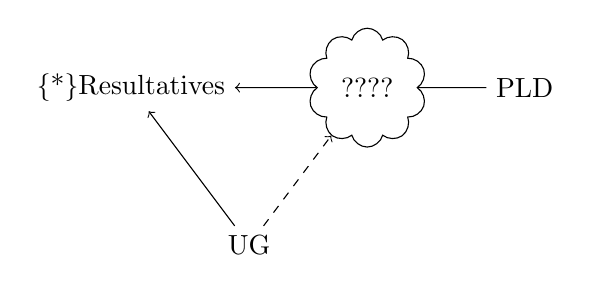
\begin{tikzpicture}
	\node (param) at (0,0) {\{*\}Resultatives};
	\node[cloud,draw] (cloud) at (3,0) {????};
	\node (PLD) at (5,0) {PLD};
	\node (UG) at (1.5,-2) {UG};
	\draw (PLD) -- (cloud);
	\draw[->] (cloud) -- (param);
	\draw[->] (UG) -- (param);
	\draw[->,dashed] (UG) -- (cloud);
      \end{tikzpicture}
      \caption{Acquiring Resultatives}
      \label{fig:resAcq}
    \end{figure}
  \end{overprint}
\end{frame}
\begin{frame}
  \begin{block}
    {My Thesis Project:}
    \begin{itemize}
      \item Explaining how a semantic ``parameter setting'' can be acquired from surface phenomena in the PLD.
    \end{itemize}
    \onslide<2>{
      In other words:
    \begin{itemize}
      \item Figuring out what's behind those question marks.
    \end{itemize}}
  \end{block}
  \onslide<2>{
      \centering
      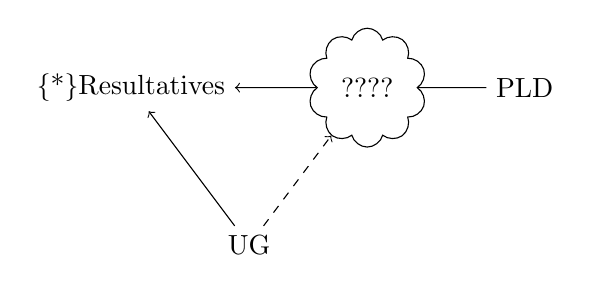
\begin{tikzpicture}
	\node (param) at (0,0) {\{*\}Resultatives};
	\node[cloud,draw] (cloud) at (3,0) {????};
	\node (PLD) at (5,0) {PLD};
	\node (UG) at (1.5,-2) {UG};
	\draw (PLD) -- (cloud);
	\draw[->] (cloud) -- (param);
	\draw[->] (UG) -- (param);
	\draw[->,dashed] (UG) -- (cloud);
      \end{tikzpicture}
  }
\end{frame}
\section{How will I explain it?}
\begin{frame}
  \frametitle{Ingredients of an explanation}
  \begin{enumerate}
    \item The surface phnomena associated with \{*\}Resultatives.
    \item A structural analysis of resultatives.
    \item A way of linking the first two ingredients.
  \end{enumerate}
\end{frame}<++>
\end{document}
